\documentclass[twoside]{book}

% Packages required by doxygen
\usepackage{calc}
\usepackage{doxygen}
\usepackage{graphicx}
\usepackage[utf8]{inputenc}
\usepackage{makeidx}
\usepackage{multicol}
\usepackage{multirow}
\usepackage{textcomp}
\usepackage[table]{xcolor}

% Font selection
\usepackage[T1]{fontenc}
\usepackage{mathptmx}
\usepackage[scaled=.90]{helvet}
\usepackage{courier}
\usepackage{amssymb}
\usepackage{sectsty}
\renewcommand{\familydefault}{\sfdefault}
\allsectionsfont{%
  \fontseries{bc}\selectfont%
  \color{darkgray}%
}
\renewcommand{\DoxyLabelFont}{%
  \fontseries{bc}\selectfont%
  \color{darkgray}%
}

% Page & text layout
\usepackage{geometry}
\geometry{%
  a4paper,%
  top=2.5cm,%
  bottom=2.5cm,%
  left=2.5cm,%
  right=2.5cm%
}
\tolerance=750
\hfuzz=15pt
\hbadness=750
\setlength{\emergencystretch}{15pt}
\setlength{\parindent}{0cm}
\setlength{\parskip}{0.2cm}
\makeatletter
\renewcommand{\paragraph}{%
  \@startsection{paragraph}{4}{0ex}{-1.0ex}{1.0ex}{%
    \normalfont\normalsize\bfseries\SS@parafont%
  }%
}
\renewcommand{\subparagraph}{%
  \@startsection{subparagraph}{5}{0ex}{-1.0ex}{1.0ex}{%
    \normalfont\normalsize\bfseries\SS@subparafont%
  }%
}
\makeatother

% Headers & footers
\usepackage{fancyhdr}
\pagestyle{fancyplain}
\fancyhead[LE]{\fancyplain{}{\bfseries\thepage}}
\fancyhead[CE]{\fancyplain{}{}}
\fancyhead[RE]{\fancyplain{}{\bfseries\leftmark}}
\fancyhead[LO]{\fancyplain{}{\bfseries\rightmark}}
\fancyhead[CO]{\fancyplain{}{}}
\fancyhead[RO]{\fancyplain{}{\bfseries\thepage}}
\fancyfoot[LE]{\fancyplain{}{}}
\fancyfoot[CE]{\fancyplain{}{}}
\fancyfoot[RE]{\fancyplain{}{\bfseries\scriptsize Generated on Mon Oct 28 2013 13\-:47\-:54 for ioskj by Doxygen }}
\fancyfoot[LO]{\fancyplain{}{\bfseries\scriptsize Generated on Mon Oct 28 2013 13\-:47\-:54 for ioskj by Doxygen }}
\fancyfoot[CO]{\fancyplain{}{}}
\fancyfoot[RO]{\fancyplain{}{}}
\renewcommand{\footrulewidth}{0.4pt}
\renewcommand{\chaptermark}[1]{%
  \markboth{#1}{}%
}
\renewcommand{\sectionmark}[1]{%
  \markright{\thesection\ #1}%
}

% Indices & bibliography
\usepackage{natbib}
\usepackage[titles]{tocloft}
\setcounter{tocdepth}{3}
\setcounter{secnumdepth}{5}
\makeindex

% Hyperlinks (required, but should be loaded last)
\usepackage{ifpdf}
\ifpdf
  \usepackage[pdftex,pagebackref=true]{hyperref}
\else
  \usepackage[ps2pdf,pagebackref=true]{hyperref}
\fi
\hypersetup{%
  colorlinks=true,%
  linkcolor=blue,%
  citecolor=blue,%
  unicode%
}

% Custom commands
\newcommand{\clearemptydoublepage}{%
  \newpage{\pagestyle{empty}\cleardoublepage}%
}


%===== C O N T E N T S =====

\begin{document}

% Titlepage & ToC
\hypersetup{pageanchor=false}
\pagenumbering{roman}
\begin{titlepage}
\vspace*{7cm}
\begin{center}%
{\Large ioskj }\\
\vspace*{1cm}
{\large Generated by Doxygen 1.8.5}\\
\vspace*{0.5cm}
{\small Mon Oct 28 2013 13:47:54}\\
\end{center}
\end{titlepage}
\clearemptydoublepage
\tableofcontents
\clearemptydoublepage
\pagenumbering{arabic}
\hypersetup{pageanchor=true}

%--- Begin generated contents ---
\chapter{Test List}
\label{test}
\hypertarget{test}{}

\begin{DoxyRefList}
\item[\label{test__test000001}%
\hypertarget{test__test000001}{}%
Class \hyperlink{classIOSKJ_1_1Model}{I\-O\-S\-K\-J\-:\-:Model} ]equilibrium\-\_\-stable

equilibrium\-\_\-uniform

recruiment\-\_\-variation

exploitation\-\_\-specified
\end{DoxyRefList}
\chapter{Todo List}
\label{todo}
\hypertarget{todo}{}

\begin{DoxyRefList}
\item[\label{todo__todo000002}%
\hypertarget{todo__todo000002}{}%
Member \hyperlink{classIOSKJ_1_1Model_af163ebda22001c7df308dc227c1687bb}{I\-O\-S\-K\-J\-:\-:Model\-:\-:step} (void)]check this equation 
\end{DoxyRefList}
\chapter{Hierarchical Index}
\section{Class Hierarchy}
This inheritance list is sorted roughly, but not completely, alphabetically\-:\begin{DoxyCompactList}
\item Data\-Group\begin{DoxyCompactList}
\item \contentsline{section}{I\-O\-S\-K\-J\-:\-:Data}{\pageref{classIOSKJ_1_1Data}}{}
\end{DoxyCompactList}
\item Dimension\begin{DoxyCompactList}
\item \contentsline{section}{I\-O\-S\-K\-J\-:\-:Data\-Year}{\pageref{classIOSKJ_1_1DataYear}}{}
\item \contentsline{section}{I\-O\-S\-K\-J\-:\-:Year}{\pageref{classIOSKJ_1_1Year}}{}
\end{DoxyCompactList}
\item \contentsline{section}{I\-O\-S\-K\-J\-:\-:Model}{\pageref{classIOSKJ_1_1Model}}{}
\item \contentsline{section}{model\-Fixture}{\pageref{structmodelFixture}}{}
\item Parameter\-Group\begin{DoxyCompactList}
\item \contentsline{section}{I\-O\-S\-K\-J\-:\-:Parameters}{\pageref{classIOSKJ_1_1Parameters}}{}
\end{DoxyCompactList}
\item \contentsline{section}{I\-O\-S\-K\-J\-:\-:Tracker}{\pageref{structIOSKJ_1_1Tracker}}{}
\end{DoxyCompactList}

\chapter{Class Index}
\section{Class List}
Here are the classes, structs, unions and interfaces with brief descriptions\-:\begin{DoxyCompactList}
\item\contentsline{section}{\hyperlink{classIOSKJ_1_1Fish}{I\-O\-S\-K\-J\-::\-Fish} }{\pageref{classIOSKJ_1_1Fish}}{}
\item\contentsline{section}{\hyperlink{classIOSKJ_1_1Fishing}{I\-O\-S\-K\-J\-::\-Fishing} }{\pageref{classIOSKJ_1_1Fishing}}{}
\item\contentsline{section}{\hyperlink{structGenerator}{Generator} }{\pageref{structGenerator}}{}
\item\contentsline{section}{\hyperlink{classIOSKJ_1_1Data_1_1MaldivePlCpue}{I\-O\-S\-K\-J\-::\-Data\-::\-Maldive\-Pl\-Cpue} }{\pageref{classIOSKJ_1_1Data_1_1MaldivePlCpue}}{}
\item\contentsline{section}{\hyperlink{classIOSKJ_1_1Model}{I\-O\-S\-K\-J\-::\-Model} }{\pageref{classIOSKJ_1_1Model}}{}
\item\contentsline{section}{\hyperlink{classIOSKJ_1_1Data_1_1NominalCatch}{I\-O\-S\-K\-J\-::\-Data\-::\-Nominal\-Catch} }{\pageref{classIOSKJ_1_1Data_1_1NominalCatch}}{}
\item\contentsline{section}{\hyperlink{classIOSKJ_1_1Data_1_1SizeFrequency}{I\-O\-S\-K\-J\-::\-Data\-::\-Size\-Frequency} }{\pageref{classIOSKJ_1_1Data_1_1SizeFrequency}}{}
\item\contentsline{section}{\hyperlink{classIOSKJ_1_1Data_1_1WestPsCpue}{I\-O\-S\-K\-J\-::\-Data\-::\-West\-Ps\-Cpue} }{\pageref{classIOSKJ_1_1Data_1_1WestPsCpue}}{}
\item\contentsline{section}{\hyperlink{classIOSKJ_1_1Data_1_1ZEstimate}{I\-O\-S\-K\-J\-::\-Data\-::\-Z\-Estimate} }{\pageref{classIOSKJ_1_1Data_1_1ZEstimate}}{}
\end{DoxyCompactList}

\chapter{Class Documentation}
\hypertarget{classSpline_1_1Element}{\section{Spline$<$ X, Y $>$\-:\-:Element Class Reference}
\label{classSpline_1_1Element}\index{Spline$<$ X, Y $>$\-::\-Element@{Spline$<$ X, Y $>$\-::\-Element}}
}
\subsection*{Public Member Functions}
\begin{DoxyCompactItemize}
\item 
\hypertarget{classSpline_1_1Element_a695c4dd8fdc435c30a6f57af535940ee}{{\bfseries Element} (X \-\_\-x)}\label{classSpline_1_1Element_a695c4dd8fdc435c30a6f57af535940ee}

\item 
\hypertarget{classSpline_1_1Element_a7e96953dd79b35946450917573853999}{{\bfseries Element} (X \-\_\-x, Y \-\_\-a, Y \-\_\-b, Y \-\_\-c, Y \-\_\-d)}\label{classSpline_1_1Element_a7e96953dd79b35946450917573853999}

\item 
\hypertarget{classSpline_1_1Element_a7311d21fcf5c5ddf6650d50a3068d2d4}{Y {\bfseries eval} (const X \&xx) const }\label{classSpline_1_1Element_a7311d21fcf5c5ddf6650d50a3068d2d4}

\item 
\hypertarget{classSpline_1_1Element_a8852e43590a6a049a8ea1d2d4bf5a815}{bool {\bfseries operator$<$} (const \hyperlink{classSpline_1_1Element}{Element} \&e) const }\label{classSpline_1_1Element_a8852e43590a6a049a8ea1d2d4bf5a815}

\item 
\hypertarget{classSpline_1_1Element_af6975df6a1a988f2b154758097f334d4}{bool {\bfseries operator$<$} (const X \&xx) const }\label{classSpline_1_1Element_af6975df6a1a988f2b154758097f334d4}

\end{DoxyCompactItemize}
\subsection*{Public Attributes}
\begin{DoxyCompactItemize}
\item 
\hypertarget{classSpline_1_1Element_a25cad79ff1314448e9af26e9842d72b8}{X {\bfseries x}}\label{classSpline_1_1Element_a25cad79ff1314448e9af26e9842d72b8}

\item 
\hypertarget{classSpline_1_1Element_a592445ec2cd3d32aaebfe290f7d875da}{Y {\bfseries a}}\label{classSpline_1_1Element_a592445ec2cd3d32aaebfe290f7d875da}

\item 
\hypertarget{classSpline_1_1Element_af109f201661f37626a794b1e3a55510a}{Y {\bfseries b}}\label{classSpline_1_1Element_af109f201661f37626a794b1e3a55510a}

\item 
\hypertarget{classSpline_1_1Element_ac07e9001f265749c4911309db45fd683}{Y {\bfseries c}}\label{classSpline_1_1Element_ac07e9001f265749c4911309db45fd683}

\item 
\hypertarget{classSpline_1_1Element_aea979df0cc618ad6b04c4aef4d8bcbb0}{Y {\bfseries d}}\label{classSpline_1_1Element_aea979df0cc618ad6b04c4aef4d8bcbb0}

\end{DoxyCompactItemize}


The documentation for this class was generated from the following file\-:\begin{DoxyCompactItemize}
\item 
spline.\-hpp\end{DoxyCompactItemize}

\hypertarget{structGenerator}{\section{Generator Struct Reference}
\label{structGenerator}\index{Generator@{Generator}}
}


{\ttfamily \#include $<$distributions.\-hpp$>$}

Inheritance diagram for Generator\-:\begin{figure}[H]
\begin{center}
\leavevmode
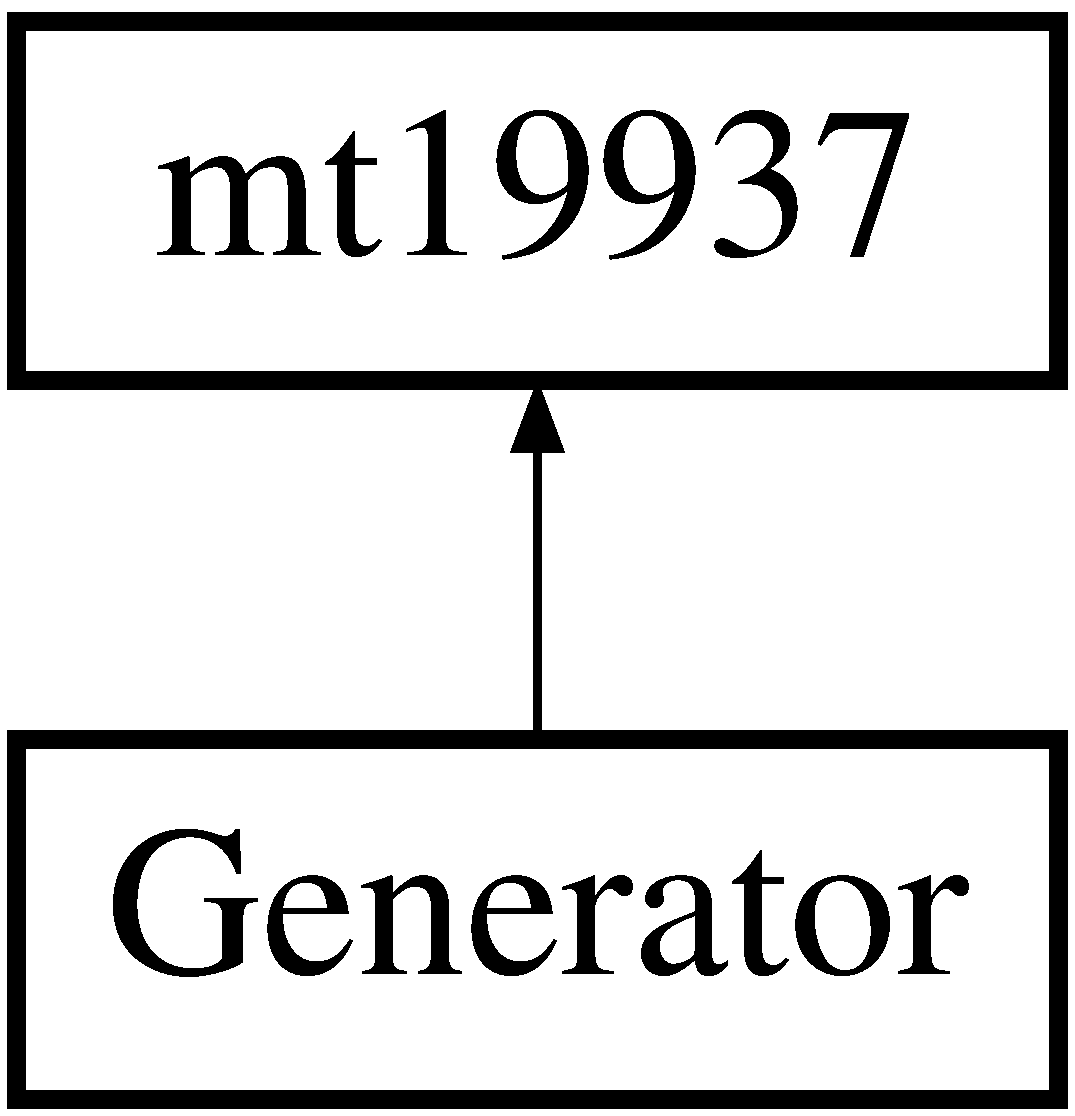
\includegraphics[height=2.000000cm]{structGenerator}
\end{center}
\end{figure}
\subsection*{Public Member Functions}
\begin{DoxyCompactItemize}
\item 
\hyperlink{structGenerator_a35e61989f22dfc623b2237ece2436dd4}{Generator} (void)
\end{DoxyCompactItemize}


\subsection{Detailed Description}
A scaffolding object that holds the random number generator used in the random() methods 

\subsection{Constructor \& Destructor Documentation}
\hypertarget{structGenerator_a35e61989f22dfc623b2237ece2436dd4}{\index{Generator@{Generator}!Generator@{Generator}}
\index{Generator@{Generator}!Generator@{Generator}}
\subsubsection[{Generator}]{\setlength{\rightskip}{0pt plus 5cm}Generator\-::\-Generator (
\begin{DoxyParamCaption}
\item[{void}]{}
\end{DoxyParamCaption}
)\hspace{0.3cm}{\ttfamily [inline]}}}\label{structGenerator_a35e61989f22dfc623b2237ece2436dd4}
Set random number generator seed using current time 

The documentation for this struct was generated from the following file\-:\begin{DoxyCompactItemize}
\item 
/home/nbentley/\-Trophia/\-Code/ioskj/distributions.\-hpp\end{DoxyCompactItemize}

\hypertarget{classIOSKJ_1_1Data_1_1MaldivePlCpue}{\section{I\-O\-S\-K\-J\-:\-:Data\-:\-:Maldive\-Pl\-Cpue Class Reference}
\label{classIOSKJ_1_1Data_1_1MaldivePlCpue}\index{I\-O\-S\-K\-J\-::\-Data\-::\-Maldive\-Pl\-Cpue@{I\-O\-S\-K\-J\-::\-Data\-::\-Maldive\-Pl\-Cpue}}
}
\subsection*{Public Member Functions}
\begin{DoxyCompactItemize}
\item 
\hypertarget{classIOSKJ_1_1Data_1_1MaldivePlCpue_a70c9b6be419fdb294f308ea5daa86aa9}{void {\bfseries read} (std\-::istream \&stream)}\label{classIOSKJ_1_1Data_1_1MaldivePlCpue_a70c9b6be419fdb294f308ea5daa86aa9}

\item 
\hypertarget{classIOSKJ_1_1Data_1_1MaldivePlCpue_a5cc13990332eef94093c2b0d4c4ac150}{void {\bfseries write} (std\-::ostream \&stream)}\label{classIOSKJ_1_1Data_1_1MaldivePlCpue_a5cc13990332eef94093c2b0d4c4ac150}

\end{DoxyCompactItemize}
\subsection*{Public Attributes}
\begin{DoxyCompactItemize}
\item 
\hypertarget{classIOSKJ_1_1Data_1_1MaldivePlCpue_a74f457be89bb489478b9361f716e52ba}{unsigned short int {\bfseries year}}\label{classIOSKJ_1_1Data_1_1MaldivePlCpue_a74f457be89bb489478b9361f716e52ba}

\item 
\hypertarget{classIOSKJ_1_1Data_1_1MaldivePlCpue_a0a933e24599d452dd116855374876bc9}{unsigned short int {\bfseries quarter}}\label{classIOSKJ_1_1Data_1_1MaldivePlCpue_a0a933e24599d452dd116855374876bc9}

\item 
\hypertarget{classIOSKJ_1_1Data_1_1MaldivePlCpue_a217bc0b50e0910ead7e0db2cbb26dc30}{float {\bfseries index}}\label{classIOSKJ_1_1Data_1_1MaldivePlCpue_a217bc0b50e0910ead7e0db2cbb26dc30}

\end{DoxyCompactItemize}


The documentation for this class was generated from the following file\-:\begin{DoxyCompactItemize}
\item 
data.\-hpp\end{DoxyCompactItemize}

\hypertarget{classIOSKJ_1_1Model}{\section{I\-O\-S\-K\-J\-:\-:Model Class Reference}
\label{classIOSKJ_1_1Model}\index{I\-O\-S\-K\-J\-::\-Model@{I\-O\-S\-K\-J\-::\-Model}}
}
\subsection*{Public Member Functions}
\begin{DoxyCompactItemize}
\item 
\hypertarget{classIOSKJ_1_1Model_ae261a53c42f71d17182c1b129698126d}{void {\bfseries track\-\_\-begin} (void)}\label{classIOSKJ_1_1Model_ae261a53c42f71d17182c1b129698126d}

\item 
\hypertarget{classIOSKJ_1_1Model_af18a3687dd2685745174b91e0aae56ce}{void {\bfseries track} (void)}\label{classIOSKJ_1_1Model_af18a3687dd2685745174b91e0aae56ce}

\item 
\hypertarget{classIOSKJ_1_1Model_a03e6aeb637c83c34774ac66c18bac74d}{void {\bfseries track\-\_\-end} (void)}\label{classIOSKJ_1_1Model_a03e6aeb637c83c34774ac66c18bac74d}

\item 
\hypertarget{classIOSKJ_1_1Model_a6f42bfc7352faa7bba7e00d04fc166b0}{void {\bfseries startup} (void)}\label{classIOSKJ_1_1Model_a6f42bfc7352faa7bba7e00d04fc166b0}

\item 
\hypertarget{classIOSKJ_1_1Model_abf9ebdb10aee501808836438cb542fab}{void {\bfseries simulate} (void)}\label{classIOSKJ_1_1Model_abf9ebdb10aee501808836438cb542fab}

\item 
\hypertarget{classIOSKJ_1_1Model_a343216d7c9019f15f01f205423001005}{void {\bfseries shutdown} (void)}\label{classIOSKJ_1_1Model_a343216d7c9019f15f01f205423001005}

\end{DoxyCompactItemize}
\subsection*{Public Attributes}
\begin{DoxyCompactItemize}
\item 
\hypertarget{classIOSKJ_1_1Model_aa8bf5f43996857e428bb0745943363a4}{\hyperlink{classIOSKJ_1_1Fish}{Fish} {\bfseries fish}}\label{classIOSKJ_1_1Model_aa8bf5f43996857e428bb0745943363a4}

\item 
\hypertarget{classIOSKJ_1_1Model_a416c537ca8c64648516e928fcea72ef2}{\hyperlink{classIOSKJ_1_1Fishing}{Fishing} {\bfseries fishing}}\label{classIOSKJ_1_1Model_a416c537ca8c64648516e928fcea72ef2}

\end{DoxyCompactItemize}


The documentation for this class was generated from the following file\-:\begin{DoxyCompactItemize}
\item 
/home/nbentley/\-Trophia/\-Code/ioskj/model.\-hpp\end{DoxyCompactItemize}

\hypertarget{structmodelFixture}{\section{model\-Fixture Struct Reference}
\label{structmodelFixture}\index{model\-Fixture@{model\-Fixture}}
}
\subsection*{Public Attributes}
\begin{DoxyCompactItemize}
\item 
\hypertarget{structmodelFixture_a9702da6353c7cd38b76d85270e0fea6f}{\hyperlink{classIOSKJ_1_1Model}{Model} {\bfseries model}}\label{structmodelFixture_a9702da6353c7cd38b76d85270e0fea6f}

\end{DoxyCompactItemize}


The documentation for this struct was generated from the following file\-:\begin{DoxyCompactItemize}
\item 
tests.\-cpp\end{DoxyCompactItemize}

\hypertarget{classIOSKJ_1_1Data_1_1NominalCatch}{\section{I\-O\-S\-K\-J\-:\-:Data\-:\-:Nominal\-Catch Class Reference}
\label{classIOSKJ_1_1Data_1_1NominalCatch}\index{I\-O\-S\-K\-J\-::\-Data\-::\-Nominal\-Catch@{I\-O\-S\-K\-J\-::\-Data\-::\-Nominal\-Catch}}
}
\subsection*{Public Member Functions}
\begin{DoxyCompactItemize}
\item 
\hypertarget{classIOSKJ_1_1Data_1_1NominalCatch_a951b91a43b44fe8e0ade88245627a2ad}{void {\bfseries read} (std\-::istream \&stream)}\label{classIOSKJ_1_1Data_1_1NominalCatch_a951b91a43b44fe8e0ade88245627a2ad}

\item 
\hypertarget{classIOSKJ_1_1Data_1_1NominalCatch_ae32b6f662319fa27352d89e7f5918e5a}{void {\bfseries write} (std\-::ostream \&stream)}\label{classIOSKJ_1_1Data_1_1NominalCatch_ae32b6f662319fa27352d89e7f5918e5a}

\end{DoxyCompactItemize}
\subsection*{Public Attributes}
\begin{DoxyCompactItemize}
\item 
\hypertarget{classIOSKJ_1_1Data_1_1NominalCatch_a44e0f37b2fca0167eb89c4eea98785f3}{char {\bfseries area}}\label{classIOSKJ_1_1Data_1_1NominalCatch_a44e0f37b2fca0167eb89c4eea98785f3}

\item 
\hypertarget{classIOSKJ_1_1Data_1_1NominalCatch_a7c81dbf0ee1c934b6dad81477365a04e}{std\-::string {\bfseries method}}\label{classIOSKJ_1_1Data_1_1NominalCatch_a7c81dbf0ee1c934b6dad81477365a04e}

\item 
\hypertarget{classIOSKJ_1_1Data_1_1NominalCatch_a2a39b5de33deffc3bdfd20acf03be16b}{unsigned short int {\bfseries year}}\label{classIOSKJ_1_1Data_1_1NominalCatch_a2a39b5de33deffc3bdfd20acf03be16b}

\item 
\hypertarget{classIOSKJ_1_1Data_1_1NominalCatch_a480209d8d8f192a933a38aa872733131}{unsigned short int {\bfseries quarter}}\label{classIOSKJ_1_1Data_1_1NominalCatch_a480209d8d8f192a933a38aa872733131}

\item 
\hypertarget{classIOSKJ_1_1Data_1_1NominalCatch_afdcdb166bea101d81920b8508d785ebe}{float {\bfseries catches}}\label{classIOSKJ_1_1Data_1_1NominalCatch_afdcdb166bea101d81920b8508d785ebe}

\end{DoxyCompactItemize}


The documentation for this class was generated from the following file\-:\begin{DoxyCompactItemize}
\item 
data.\-hpp\end{DoxyCompactItemize}

\hypertarget{classIOSKJ_1_1Data_1_1SizeFrequency}{\section{I\-O\-S\-K\-J\-:\-:Data\-:\-:Size\-Frequency Class Reference}
\label{classIOSKJ_1_1Data_1_1SizeFrequency}\index{I\-O\-S\-K\-J\-::\-Data\-::\-Size\-Frequency@{I\-O\-S\-K\-J\-::\-Data\-::\-Size\-Frequency}}
}
\subsection*{Public Member Functions}
\begin{DoxyCompactItemize}
\item 
\hypertarget{classIOSKJ_1_1Data_1_1SizeFrequency_a47ab1ffa698fd8b3158eec2451a07b99}{void {\bfseries read} (std\-::istream \&stream)}\label{classIOSKJ_1_1Data_1_1SizeFrequency_a47ab1ffa698fd8b3158eec2451a07b99}

\item 
\hypertarget{classIOSKJ_1_1Data_1_1SizeFrequency_ae75970f485f011f5191566ca0987c572}{void {\bfseries write} (std\-::ostream \&stream)}\label{classIOSKJ_1_1Data_1_1SizeFrequency_ae75970f485f011f5191566ca0987c572}

\end{DoxyCompactItemize}
\subsection*{Public Attributes}
\begin{DoxyCompactItemize}
\item 
\hypertarget{classIOSKJ_1_1Data_1_1SizeFrequency_a08b0a6bd3c85e65f42521048e6e3bab3}{char {\bfseries area}}\label{classIOSKJ_1_1Data_1_1SizeFrequency_a08b0a6bd3c85e65f42521048e6e3bab3}

\item 
\hypertarget{classIOSKJ_1_1Data_1_1SizeFrequency_a49c0a08a3422004645d2226265c237c7}{std\-::string {\bfseries method}}\label{classIOSKJ_1_1Data_1_1SizeFrequency_a49c0a08a3422004645d2226265c237c7}

\item 
\hypertarget{classIOSKJ_1_1Data_1_1SizeFrequency_a19ef92240e288f489c5d90b1c4df0000}{unsigned short int {\bfseries year}}\label{classIOSKJ_1_1Data_1_1SizeFrequency_a19ef92240e288f489c5d90b1c4df0000}

\item 
\hypertarget{classIOSKJ_1_1Data_1_1SizeFrequency_aee8e747384c06491bebb7cc539bbb15a}{unsigned short int {\bfseries quarter}}\label{classIOSKJ_1_1Data_1_1SizeFrequency_aee8e747384c06491bebb7cc539bbb15a}

\item 
\hypertarget{classIOSKJ_1_1Data_1_1SizeFrequency_ab9833e7a7783b8b73489ac83ad0d4bd8}{std\-::array$<$ float, 61 $>$ {\bfseries props}}\label{classIOSKJ_1_1Data_1_1SizeFrequency_ab9833e7a7783b8b73489ac83ad0d4bd8}

\item 
\hypertarget{classIOSKJ_1_1Data_1_1SizeFrequency_ad494b63b6b89bdedae41e62ce4dbc1d7}{unsigned int {\bfseries num}}\label{classIOSKJ_1_1Data_1_1SizeFrequency_ad494b63b6b89bdedae41e62ce4dbc1d7}

\end{DoxyCompactItemize}


The documentation for this class was generated from the following file\-:\begin{DoxyCompactItemize}
\item 
data.\-hpp\end{DoxyCompactItemize}

\hypertarget{classSpline}{\section{Spline$<$ X, Y $>$ Class Template Reference}
\label{classSpline}\index{Spline$<$ X, Y $>$@{Spline$<$ X, Y $>$}}
}


{\ttfamily \#include $<$spline.\-hpp$>$}

\subsection*{Classes}
\begin{DoxyCompactItemize}
\item 
class \hyperlink{classSpline_1_1Element}{Element}
\end{DoxyCompactItemize}
\subsection*{Public Member Functions}
\begin{DoxyCompactItemize}
\item 
\hypertarget{classSpline_a9202b2897674c1877b2287f83a3079e9}{{\bfseries Spline} (const std\-::vector$<$ X $>$ \&x, const std\-::vector$<$ Y $>$ \&y)}\label{classSpline_a9202b2897674c1877b2287f83a3079e9}

\item 
\hypertarget{classSpline_a5297f90ac8e0b4758e88b7b4cecf2633}{\hyperlink{classSpline}{Spline} \& {\bfseries knots} (const std\-::vector$<$ X $>$ \&x, const std\-::vector$<$ Y $>$ \&y)}\label{classSpline_a5297f90ac8e0b4758e88b7b4cecf2633}

\item 
\hypertarget{classSpline_a52fd94178e1e0cb612bdb018acc1fee6}{Y {\bfseries operator\mbox{[}$\,$\mbox{]}} (const X \&x) const }\label{classSpline_a52fd94178e1e0cb612bdb018acc1fee6}

\item 
\hypertarget{classSpline_ad8594d762a6673e573d38aba5bef70ec}{Y {\bfseries interpolate} (const X \&x) const }\label{classSpline_ad8594d762a6673e573d38aba5bef70ec}

\item 
\hypertarget{classSpline_abdd648dce89434bacb38309eadf13106}{std\-::vector$<$ Y $>$ {\bfseries operator\mbox{[}$\,$\mbox{]}} (const std\-::vector$<$ X $>$ \&xx) const }\label{classSpline_abdd648dce89434bacb38309eadf13106}

\item 
\hypertarget{classSpline_aec162530d74514a6bc57d1cd8d7fe116}{std\-::vector$<$ Y $>$ {\bfseries interpolate} (const std\-::vector$<$ X $>$ \&xx) const }\label{classSpline_aec162530d74514a6bc57d1cd8d7fe116}

\end{DoxyCompactItemize}
\subsection*{Protected Types}
\begin{DoxyCompactItemize}
\item 
\hypertarget{classSpline_a0e5f568df00822e6467ad4b6ae6907f1}{typedef \hyperlink{classSpline_1_1Element}{Element} {\bfseries element\-\_\-type}}\label{classSpline_a0e5f568df00822e6467ad4b6ae6907f1}

\end{DoxyCompactItemize}
\subsection*{Protected Attributes}
\begin{DoxyCompactItemize}
\item 
\hypertarget{classSpline_aec12d605758ea834a7de781781de7e95}{std\-::vector$<$ \hyperlink{classSpline_1_1Element}{element\-\_\-type} $>$ {\bfseries m\-Elements}}\label{classSpline_aec12d605758ea834a7de781781de7e95}

\end{DoxyCompactItemize}


\subsection{Detailed Description}
\subsubsection*{template$<$typename X, typename Y$>$class Spline$<$ X, Y $>$}

Cubic spline interpolation class from \href{http://shiftedbits.org/2011/01/30/cubic-spline-interpolation/}{\tt http\-://shiftedbits.\-org/2011/01/30/cubic-\/spline-\/interpolation/}

Modified slightly to add particular interfaces. Implementation not changed. Templated on type of X, Y. X and Y must have operator +, -\/, $\ast$, /. Y must have defined a constructor that takes a scalar. 

The documentation for this class was generated from the following file\-:\begin{DoxyCompactItemize}
\item 
spline.\-hpp\end{DoxyCompactItemize}

\hypertarget{classIOSKJ_1_1Data_1_1WestPsCpue}{\section{I\-O\-S\-K\-J\-:\-:Data\-:\-:West\-Ps\-Cpue Class Reference}
\label{classIOSKJ_1_1Data_1_1WestPsCpue}\index{I\-O\-S\-K\-J\-::\-Data\-::\-West\-Ps\-Cpue@{I\-O\-S\-K\-J\-::\-Data\-::\-West\-Ps\-Cpue}}
}
\subsection*{Public Member Functions}
\begin{DoxyCompactItemize}
\item 
\hypertarget{classIOSKJ_1_1Data_1_1WestPsCpue_a4a66b4d327983bbcc8262cae217c7ede}{void {\bfseries read} (std\-::istream \&stream)}\label{classIOSKJ_1_1Data_1_1WestPsCpue_a4a66b4d327983bbcc8262cae217c7ede}

\item 
\hypertarget{classIOSKJ_1_1Data_1_1WestPsCpue_a21ae334f9ae536b2624e403c3b77216f}{void {\bfseries write} (std\-::ostream \&stream)}\label{classIOSKJ_1_1Data_1_1WestPsCpue_a21ae334f9ae536b2624e403c3b77216f}

\end{DoxyCompactItemize}
\subsection*{Public Attributes}
\begin{DoxyCompactItemize}
\item 
\hypertarget{classIOSKJ_1_1Data_1_1WestPsCpue_a76ed2a7cfc9dc71cd96e979a9310a4c7}{unsigned short int {\bfseries year}}\label{classIOSKJ_1_1Data_1_1WestPsCpue_a76ed2a7cfc9dc71cd96e979a9310a4c7}

\item 
\hypertarget{classIOSKJ_1_1Data_1_1WestPsCpue_a93d81fdc1e2168e56d3c7fc1173c493a}{float {\bfseries index}}\label{classIOSKJ_1_1Data_1_1WestPsCpue_a93d81fdc1e2168e56d3c7fc1173c493a}

\end{DoxyCompactItemize}


The documentation for this class was generated from the following file\-:\begin{DoxyCompactItemize}
\item 
/home/nbentley/\-Trophia/\-Code/ioskj/data.\-hpp\end{DoxyCompactItemize}

\hypertarget{classIOSKJ_1_1Data_1_1ZEstimate}{\section{I\-O\-S\-K\-J\-:\-:Data\-:\-:Z\-Estimate Class Reference}
\label{classIOSKJ_1_1Data_1_1ZEstimate}\index{I\-O\-S\-K\-J\-::\-Data\-::\-Z\-Estimate@{I\-O\-S\-K\-J\-::\-Data\-::\-Z\-Estimate}}
}
\subsection*{Public Member Functions}
\begin{DoxyCompactItemize}
\item 
\hypertarget{classIOSKJ_1_1Data_1_1ZEstimate_afd875241b51d49785e50acc239d7806e}{void {\bfseries read} (std\-::istream \&stream)}\label{classIOSKJ_1_1Data_1_1ZEstimate_afd875241b51d49785e50acc239d7806e}

\item 
\hypertarget{classIOSKJ_1_1Data_1_1ZEstimate_a952dba16d22242db687179289e576b08}{void {\bfseries write} (std\-::ostream \&stream)}\label{classIOSKJ_1_1Data_1_1ZEstimate_a952dba16d22242db687179289e576b08}

\end{DoxyCompactItemize}
\subsection*{Public Attributes}
\begin{DoxyCompactItemize}
\item 
\hypertarget{classIOSKJ_1_1Data_1_1ZEstimate_a2511cde8860fc325a4be66a05d806b94}{unsigned short int {\bfseries year}}\label{classIOSKJ_1_1Data_1_1ZEstimate_a2511cde8860fc325a4be66a05d806b94}

\item 
\hypertarget{classIOSKJ_1_1Data_1_1ZEstimate_abc1f796aef34133f4dad711ace3dd529}{unsigned short int {\bfseries quarter}}\label{classIOSKJ_1_1Data_1_1ZEstimate_abc1f796aef34133f4dad711ace3dd529}

\item 
\hypertarget{classIOSKJ_1_1Data_1_1ZEstimate_ab3cf8c05dd916758fcc22c8676473182}{float {\bfseries mu45}}\label{classIOSKJ_1_1Data_1_1ZEstimate_ab3cf8c05dd916758fcc22c8676473182}

\item 
\hypertarget{classIOSKJ_1_1Data_1_1ZEstimate_a49b0106bd644e434504ce8c677bf5d5b}{float {\bfseries mu50}}\label{classIOSKJ_1_1Data_1_1ZEstimate_a49b0106bd644e434504ce8c677bf5d5b}

\item 
\hypertarget{classIOSKJ_1_1Data_1_1ZEstimate_a7728fcde3967717cb8342ca0b0550f5d}{float {\bfseries mu55}}\label{classIOSKJ_1_1Data_1_1ZEstimate_a7728fcde3967717cb8342ca0b0550f5d}

\item 
\hypertarget{classIOSKJ_1_1Data_1_1ZEstimate_af2cdea31b63889b691238a92bca3ce10}{float {\bfseries mu60}}\label{classIOSKJ_1_1Data_1_1ZEstimate_af2cdea31b63889b691238a92bca3ce10}

\item 
\hypertarget{classIOSKJ_1_1Data_1_1ZEstimate_ac6bf29ae6cc8e5b69d21c774b5143937}{float {\bfseries sd45}}\label{classIOSKJ_1_1Data_1_1ZEstimate_ac6bf29ae6cc8e5b69d21c774b5143937}

\item 
\hypertarget{classIOSKJ_1_1Data_1_1ZEstimate_ac04b382296b2422a61d6c6e6ceb28d84}{float {\bfseries sd50}}\label{classIOSKJ_1_1Data_1_1ZEstimate_ac04b382296b2422a61d6c6e6ceb28d84}

\item 
\hypertarget{classIOSKJ_1_1Data_1_1ZEstimate_af38b9264f644528589e2fe18750177b6}{float {\bfseries sd55}}\label{classIOSKJ_1_1Data_1_1ZEstimate_af38b9264f644528589e2fe18750177b6}

\item 
\hypertarget{classIOSKJ_1_1Data_1_1ZEstimate_a19e5b287fb0fa792569a2062c2e63e2b}{float {\bfseries sd60}}\label{classIOSKJ_1_1Data_1_1ZEstimate_a19e5b287fb0fa792569a2062c2e63e2b}

\end{DoxyCompactItemize}


The documentation for this class was generated from the following file\-:\begin{DoxyCompactItemize}
\item 
/home/nbentley/\-Trophia/\-Code/ioskj/data.\-hpp\end{DoxyCompactItemize}

%--- End generated contents ---

% Index
\newpage
\phantomsection
\addcontentsline{toc}{part}{Index}
\printindex

\end{document}
